\begin{frame}{Latent Dirichlet allocation}

  \only<1>{
    \begin{figure}
      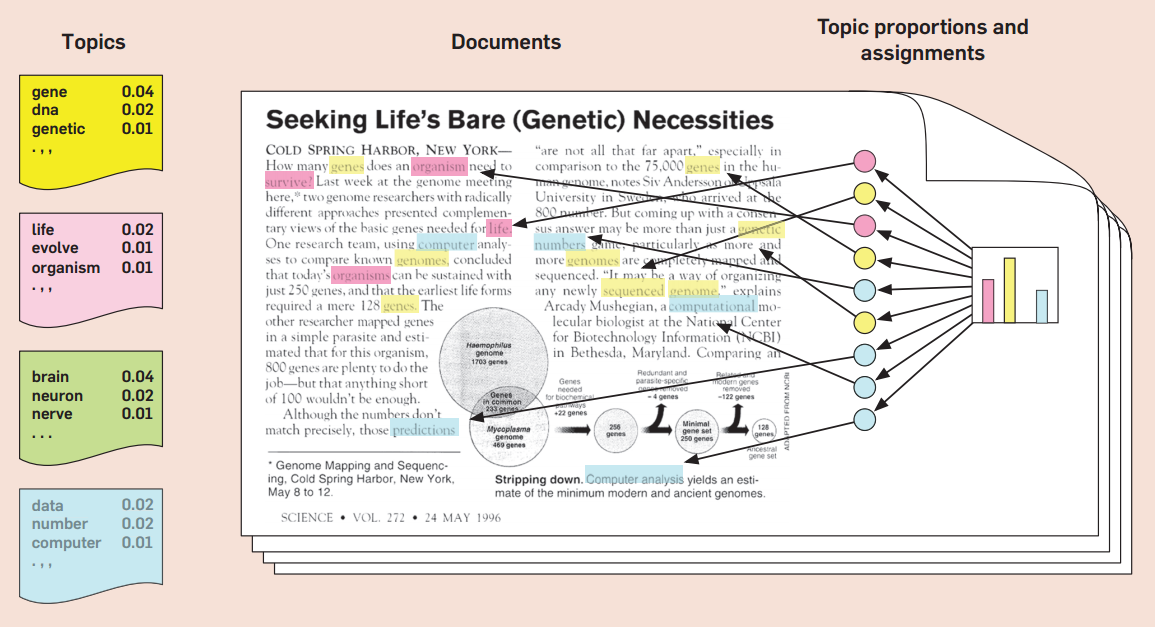
\includegraphics[width=0.8\framewidth]{figs/blei-lda.png}
      \caption{The LDA generative model.\footfullcite{Blei2012}}
    \end{figure}
  }

  \only<2>{
    \begin{align*}
      p(\beta_{1:K}, \theta_{1:D},z_{1:D} | w_{1:D}) = \frac{\beta_{1:K},
      \theta_{1:D},z_{1:D}, w_{1:D}}{w_{1:D}}
    \end{align*}

    \vfill

    Gibbs sampling is used to approximate the probability of the
    denominator (evidence)\footfullcite{Blei2012}.

    \vfill

    \begin{itemize}
      \item $\beta_{1:k} := \text{ topic } k$
      \item $\theta_{d,k} := \text{ topic proportion for topic } k \text{
      in document } d$
      \item $z_{d,n} := \text{ topic assignment for word } n \text{ in
      document } d$
      \item $w_{d,n} := \text{ the } n^{th} \text{ word in document } d$
    \end{itemize}
  }

\end{frame}
